\documentclass[tikz,border=6pt]{standalone}
\usepackage{amsmath,amssymb}
\usepackage{xcolor}
\definecolor{accent}{HTML}{A13D2C}
\definecolor{accent2}{HTML}{2B5F6B}
\definecolor{muted}{HTML}{5A564F}
\definecolor{panel}{HTML}{F8F6F0}
\definecolor{linecol}{HTML}{D8D2C4}
\definecolor{astroblue}{HTML}{1B4F72}
\definecolor{sunyellow}{HTML}{E8A33D}
\definecolor{colthree}{RGB}{60,140,80}
\usetikzlibrary{calc,arrows.meta,plotmarks}
\IfFileExists{results/ch12/lane_emden_n3.dat}{\def\datadir{results/ch12/}}{\def\datadir{../results/ch12/}}
\usepackage[T1]{fontenc}\usepackage{newpxtext,newpxmath}  % same fonts as the notes
\begin{document}
% The kappa-mechanism valve: one cycle of a layer of partly ionised helium.
% Four stages on a circle, clockwise from the top, joined by plain arrows.
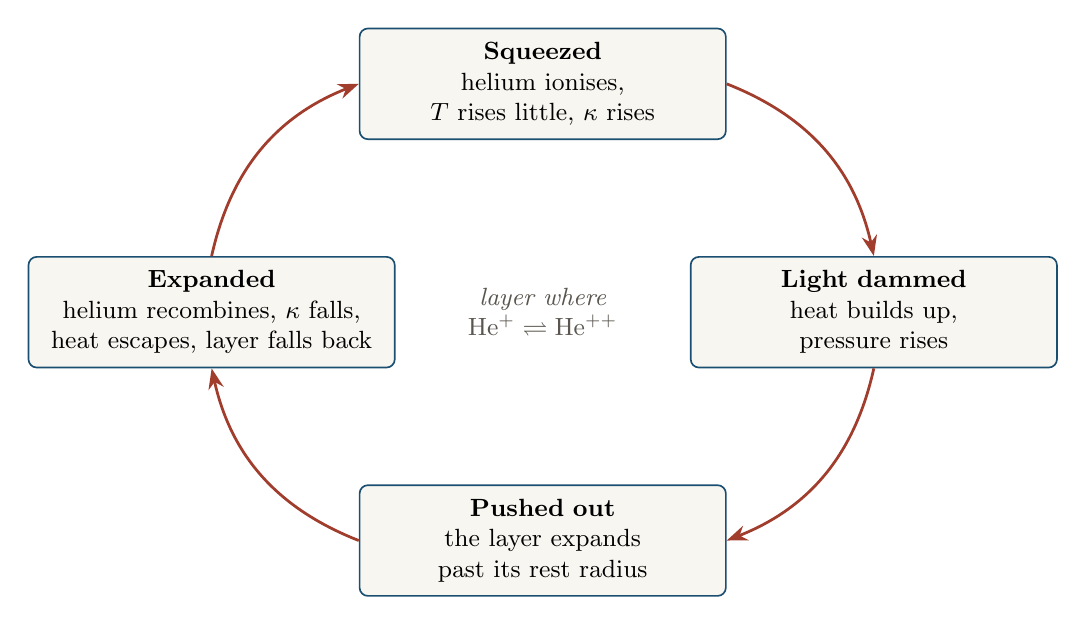
\begin{tikzpicture}[>={Stealth[length=2.6mm]}, font=\small,
  stage/.style={draw=astroblue, line width=0.6pt, fill=panel, rounded corners=3pt,
    align=center, text width=4.3cm, inner sep=5pt}]
  \def\r{2.9}
  \node[stage] (top)   at (0,\r)    {\textbf{Squeezed}\\ helium ionises,\\ $T$ rises little, $\kappa$ rises};
  \node[stage] (right) at (1.45*\r,0) {\textbf{Light dammed}\\ heat builds up,\\ pressure rises};
  \node[stage] (bot)   at (0,-\r)   {\textbf{Pushed out}\\ the layer expands\\ past its rest radius};
  \node[stage] (left)  at (-1.45*\r,0) {\textbf{Expanded}\\ helium recombines, $\kappa$ falls,\\ heat escapes, layer falls back};
  \draw[->, accent, line width=1pt] (top.east) to[bend left=28] (right.north);
  \draw[->, accent, line width=1pt] (right.south) to[bend left=28] (bot.east);
  \draw[->, accent, line width=1pt] (bot.west) to[bend left=28] (left.south);
  \draw[->, accent, line width=1pt] (left.north) to[bend left=28] (top.west);
  \node[muted, align=center, font=\small\itshape] at (0,0) {layer where\\ $\mathrm{He^+}\rightleftharpoons\mathrm{He^{++}}$};
\end{tikzpicture}
\end{document}
